\chapter{Evaluation}
\label{chap:evaluation}
	In this chapter, we asses our effort to implement the C++11 standard future interface, for 
distributed memory enviromnent, and we evaluate the performance of our runtime system.

\section{Interface Assesment}
\label{sect:interface_assesment}

\paragraph{}
Figures ~\ref{lst:fib_futures} and ~\ref{lst:fib} show an implementation of the fibonacci function using
C++11 standard futures and our futures library, respectively.  The interface used to express parallelism is
identical.  An \emph{async} call is used to send asynchronous \emph{jobs} for execution, while the return value
is encapsulated in a future object.  The return value can be retrieved in the same fashion in both libraries, 
using the get method.  Our future object behaves also like a shared\_future from the C++11 standard library,
which means that it can be accessed by different processes concurrently.  

\paragraph{}
One difference to the interfaces is that our interface requires the data size of a \emph{job}'s return 
value to be defined.  This is limited only to the case where the return value is dynamically sized object
or a pointer. 
The major difference between the two interfaces is that only functor objects can be 
issued by the \emph{async} function and that the programmer has to explicitely indentify the functors
as \emph{job}s, in order to expose their type and arguments to our runtime system.  This has minimal impact on
the user interface.  It is done very easily just by adding an extra line of code, in the example in figure 
\ref{lst:fib} this is done with 
the macro command FUTURES\_EXPORT\_FUNCTOR((async\_function<fib, int>)).  The implications of this are discussed
further in \ref{sect:interface_limitations}.  

\paragraph{}
At this moment, the interface lacks some secondary features, like defininig a launch policy and timing out
after a period of time upon waiting on a future value.  Note however, these features are trivial to implement
and of little interest to us at this point.  Another feature that we have neglected to implement is the 
ability to return an exception instead of the functor's return value.  On the other hand, we have added a couple
of features (see \ref{sect:extra_features}).  The make\_future functions can be found both in the Boost futures
library and in HPX.  Moreover, the async\_on function allows greater flexibility to the programer.  He can 
easily override the default scheduler and use a custom distribution scheme that matches his needs.  

\subsection{Limitations}
\label{sect:interface_limitations}
The core limitation of our interface is that all \emph{jobs} must be functor objects,
whereas in the C++11 standard, it is possible to use any callable object (functions, function pointer, functors,
lamda function etc.).  	This of-course, does not limit our library's expressiveness, when it comes to parallelization.
A programmer can easily wrap any callable object in a functor object.  The programmer's extra burden here is not 
note-worthy.  On the other hand,  the functor object, its return value and its arguments must be serializable, as well.  
This limitation manifests itself in our interface, both as an adittional burden to the programmer and as a potential
limitation, when porting codes with lots of pointers and maybe non-serializable objects to work with our library.
To better undersand the implications here, we share our experience when we tried to port Ferret, a benchmark from
the PARSEC~\cite{bienia11benchmarking} suite, using our library.

\paragraph{}
Ferret is a content-based similarity search engine toolkit for feature rich
data types (video, audio, images, 3D shapes, etc).
Ferret uses a pipeline model for parallelization, 
with a thread pool at each stage.  A queue exist for each stage and whenever
there is an entry on that queue, a thread from the thread pool will pop it, and start execution.  When it's
done, the tread will push an entry on the next stage's queue and so no.  This scheme can be expressed with
futures extremely easily.  Figure \ref{lst:pipe_futures_b} shows how a pipeline scheme with futures would 
look like.  We tried to implement this using both C++11 standard futures and our library.  The algorithm
was relatively easily modified to work with C++11 standard futures.  However, in order to work with our
version, we needed to modify the original queue entries, which our now the arguments to the \emph{async}
functions, in order for them to be serialiazable.  This, proved to be quite a challenge.  First, the original
code was in C language and used void* extensively.  All these pointers had to be encapsulated in 
C++ vectoer<unsigned char> objects.  The challenge here is that we needed to modify most of the functions
of the whole Ferret library, either to work with vectors instead of void pointers or simply to modify a 
number of functions to return the allocation size for each void pointer, in order to convert 
them to vector objects.  In this example, this has proven to include a large number of functions (ferret
counts more than 3000 LOC), as a result we have not yet completed its porting.  We report this in order
to show a case, where the requirment to serialize arguments, return values etc, can have a significant
impact on ease of use.  Of-couse, as a counter argument here, we have to say that it is still easier to 
use our interface instead of re-writing the whole ferret code to use a message passing library like MPI
directly.  It should also be noted, even with a message passing library, serialization or manually
manipulating the data of the void pointers would still be required.  

  
\section{Performance Evaluation}
\label{sect:eval_intro}
\paragraph{}
	We evaluated our runtime's implementation performance by running some microbenchmark applications and
three small applications (fibonacci, quicksort, LU).  We run all benchmarks on two Intel(R) Xeon(R) 
CPU E5645@2.40 GHz with with 6 available cores on each machine, totaling to 12 cores connected through 
a network socket. We have compiled the runtime and application code using g++ version 4.6.3 with 
level 3 optimizations enabled.  For the MPI library we used OpenMPI version 1.4.3.

\subsection{Microbenchmarks}
\label{sect:microbenchmark}
\paragraph{}
	Our first microbenchmark is a ping pong application, which is used to measure the time needed to send a 
message from the master to a worker node and the time needed for the worker node to respond back to the master.
Using the future interface, the master simply calls async with a functor that takes a string argument ("ping") 
and returns only a string value ("pong"), without doing any other computations in the functor's body.  We run
the ping pong microbenchmark using the configuration described in~\ref{sect:eval_intro} and the message was 
received by the master in 0.8ms.

\paragraph{}
	The rest of our microbenchmarks, aim to help us understand better the time needed to issue a job from one
node to another.  To achieve this, we designed one microbenchmark application, where the master node issues
a functor, with only a return statement in his body, which takes a variable number of arguments, each argument
can be either a scalar value or a vector container.  In figure~\ref{fig:issue_time_scalar_vs_containers} we report
the time needed to issue a job that takes a variable number of scalar arguments comparing it with the time needed
to issue a variable number of vector objects of one element.  Although the vector object arguments are more complex
to serialize, we see that the difference in execution time is marginal.  Moreover, we see that the number of arguments
has that need to be transfered, have minimal implact on execution time.  
Figure~\ref{fig:issue_time_different_argnum_same_size} shows the execution time of issuing functor objects with different
vector argument sizes.  In all cases the total number of elements totals to 1200000 (e.g. 1 vector of 1200000 elements or
4 vectors of 300000 elements).   The numbers reported are the median values of 20 runs.  The cost differences here are 
again insignificant. 

\begin{figure}[!ht]
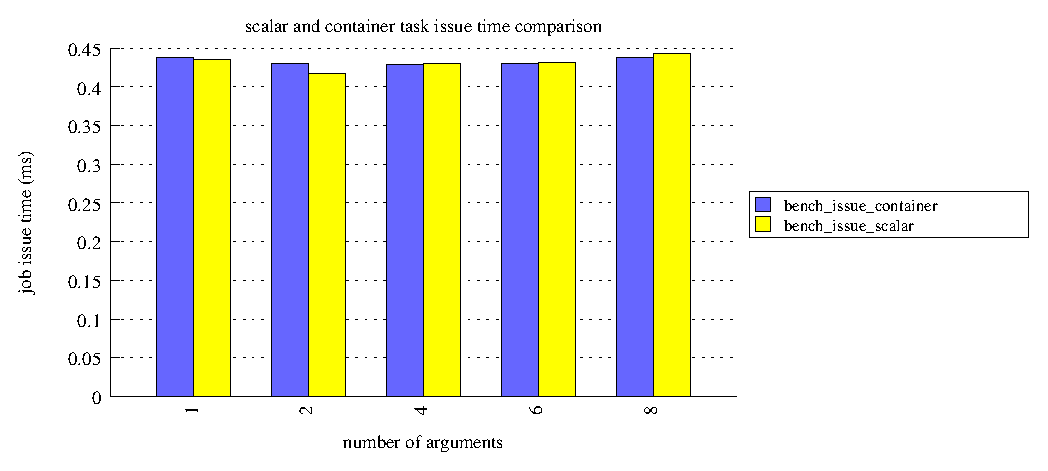
\includegraphics[width=\columnwidth]{figures/job_issue_time_scalar_vs_container_bars}
\caption{Comparison between issuing functors with scalar arguments versus vector objects of size 1}
\label{fig:issue_time_scalar_vs_containers}
\end{figure}

\begin{figure}[!ht]
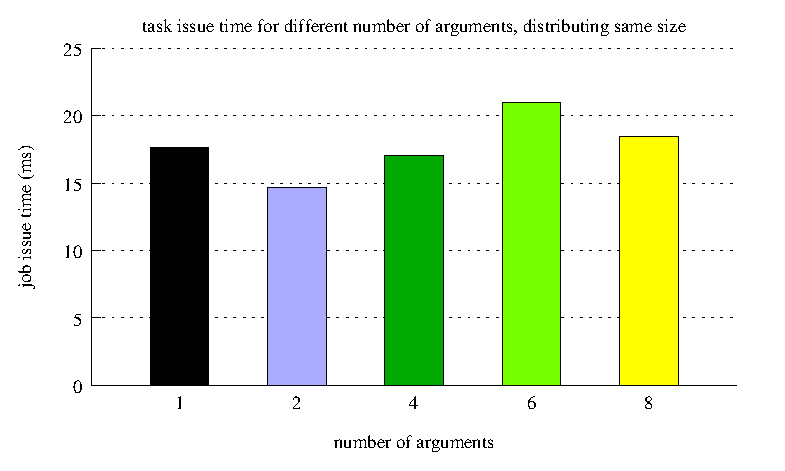
\includegraphics[width=0.7\columnwidth]{figures/job_issue_time_different_argnums_same_size_bars}
\caption{Comparison between issuing functors with different number of vector arguments, but total 
				size of arguments is the same in all cases.}
\label{fig:issue_time_different_argnum_same_size}
\end{figure}

%\begin{figure}
%	\centering
%	\begin{subfigure}[b]{0.5\textwidth}
%		\centering
%		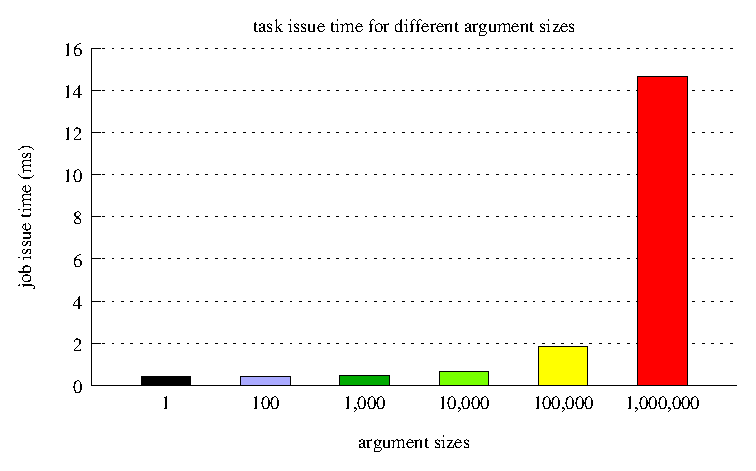
\includegraphics[width=\columnwidth]{figures/job_issue_time_different_argsizes}
%		\caption{Comparison between issuing functors with 1 vector argument of different sizes}
%		\label{fig:job_issue_time_different_argsizes}
%	\end{subfigure}%
%	~ %add desired spacing between images, e. g. ~, \quad, \qquad etc.
%		%(or a blank line to force the subfigure onto a new line)
%	\begin{subfigure}[b]{0.5\textwidth}
%		\centering
%		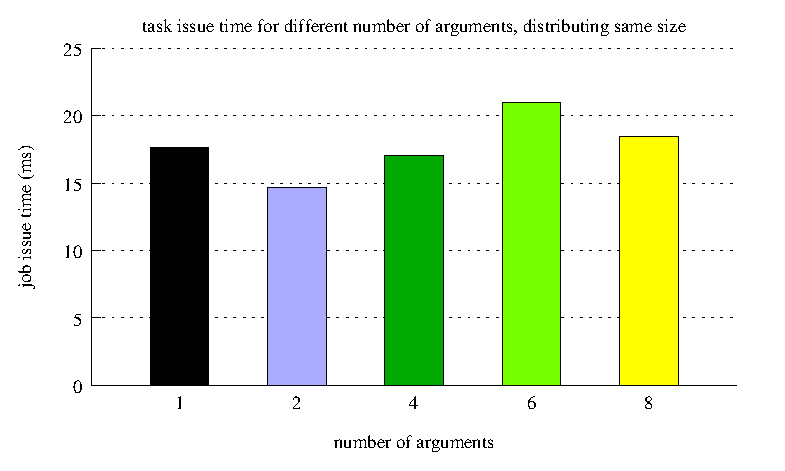
\includegraphics[width=\columnwidth]{figures/job_issue_time_different_argnums_same_size_bars}
%		\caption{Comparison between issuing functors with different number of vector arguments, but total 
%						size of arguments is the same in all cases.}
%		\label{fig:issue_time_different_argnum_same_size}
%	\end{subfigure}
%	~ %add desired spacing between images, e. g. ~, \quad, \qquad etc.
%		%(or a blank line to force the subfigure onto a new line)
%	\caption{Pictures of animals}
%	\label{fig:animals}
%\end{figure}

\begin{figure}[!ht]
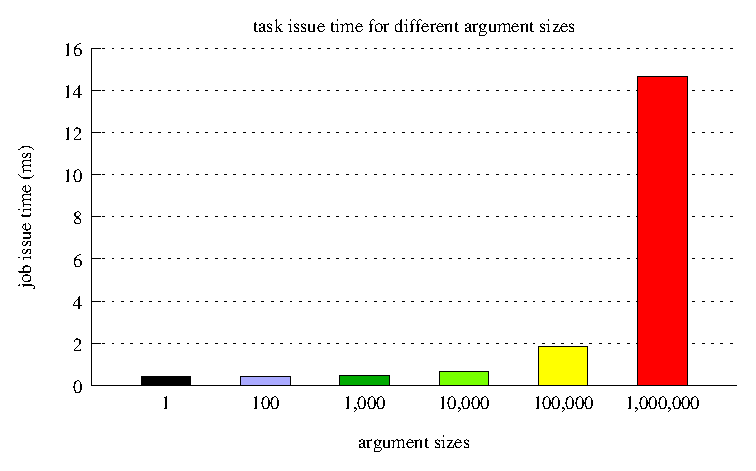
\includegraphics[width=0.7\columnwidth]{figures/job_issue_time_different_argsizes}
\caption{Comparison between issuing functors with 1 vector argument of different sizes}
\label{fig:job_issue_time_different_argsizes}
\end{figure}

\subsection{Real Application Benchmarking}
\label{sect:real_app}
\paragraph{}
	In order to evaluate our runtime's performance we have implemented three algorithms using our future's interface.

\paragraph{}
	\textbf{Fibonacci}:  This is a simple implementation of the fibonacci function.  Figure~\ref{lst:fib} shows 
our implementation.  This recursive version is ideal to demonstrate the ease of use of the future's interface.
We have modified the fibonacci code to run the sequential verson of the code for values smaller than  30, so that
each async function can have some amount of work.  We run the fibonacci function with 45 as an argument.  

\paragraph{}
	\textbf{Quicksort}:  Figure~\ref{lst:quicksort} shows our implementation.  The \emph{QsSequantial} 
function itself is a pretty standard
implementation of the common quicksort algorithm.  Parallelization is extracted at the \emph{quicksort} function, where the 
original array is partitioned and asynchrous quicksort functions are called until the \emph{min\_unit} value of elements
is reached, where from that point on the sequential version of the quicksort algorithm is called on each partition.
Notice that for the asynchronous branch of the code, we need to copy each partition in order to send it over the worker 
process and also merge the results of the async functions into the original array.  This additional overhead along with 
the communication overhead makes it necessary to sort small sub arrays sequentially.  For our experiments we sort an 
array of 100,000 doubles. 

\begin{figure}[!ht]
\center
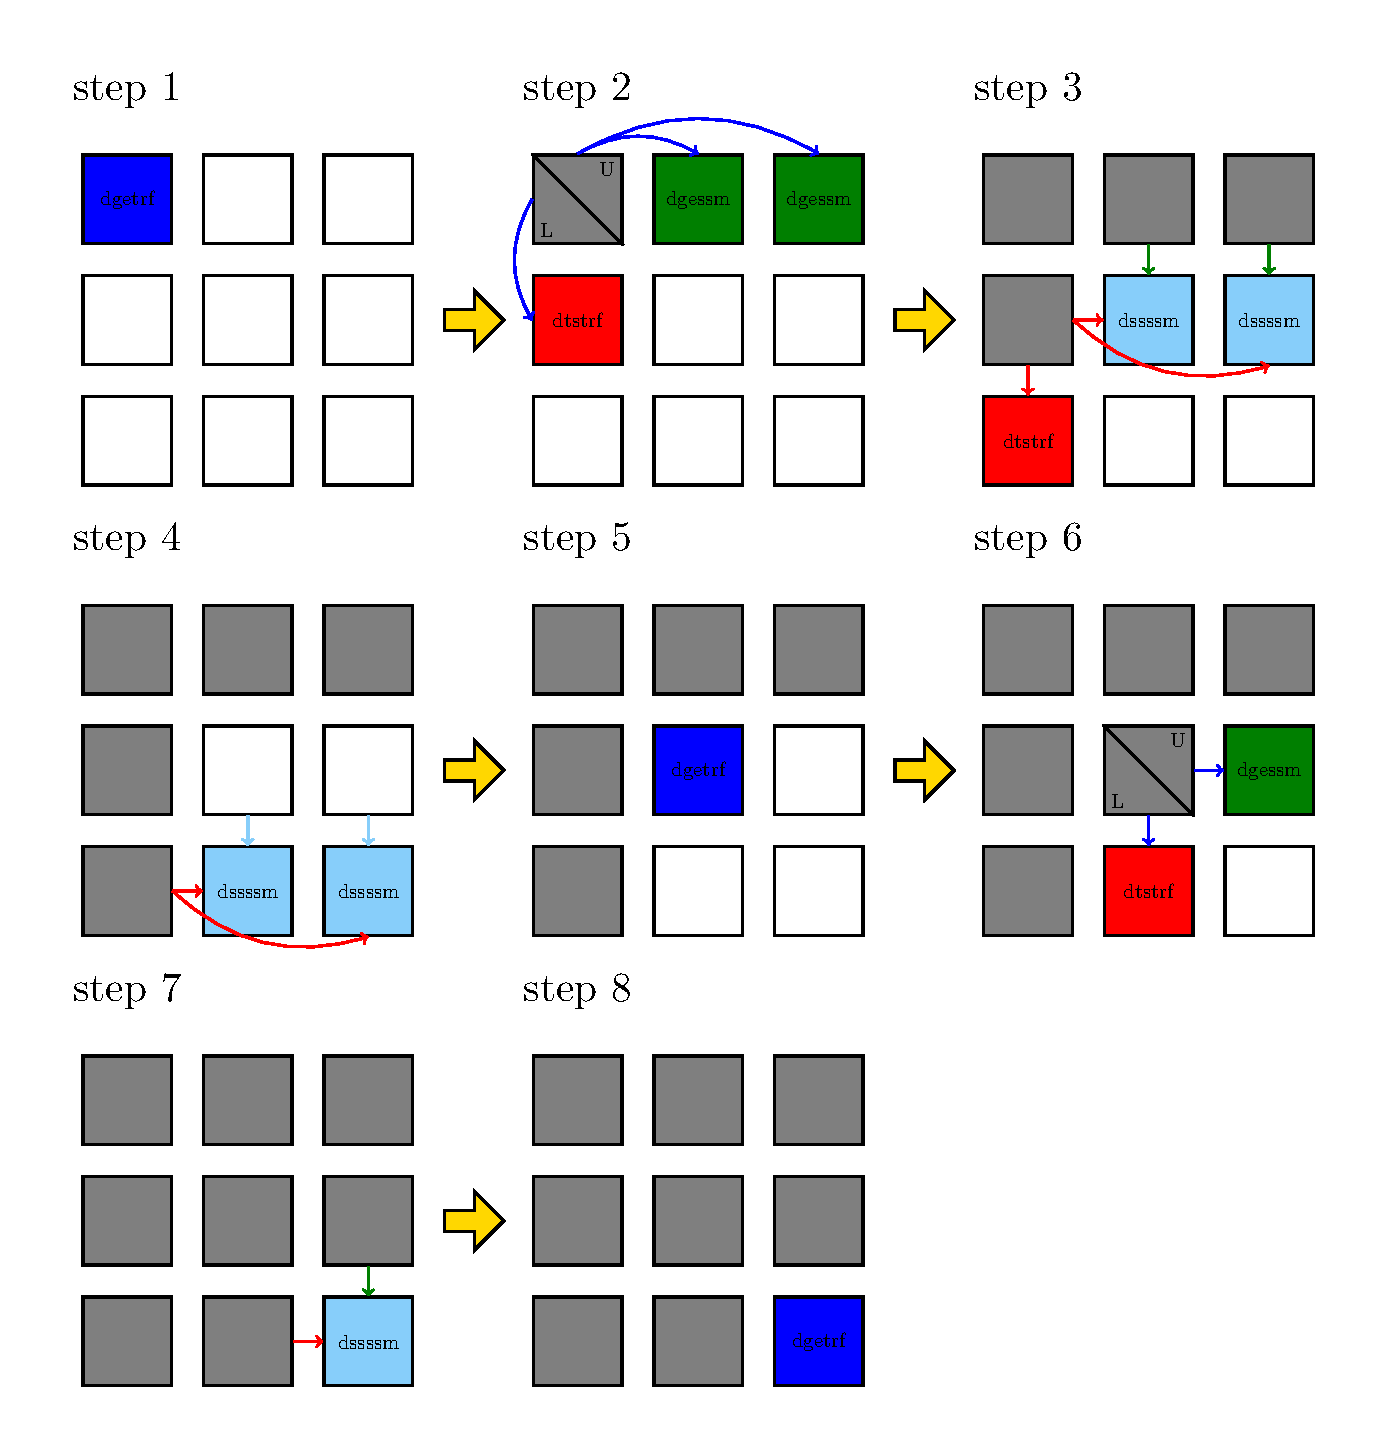
\includegraphics[width=0.8\columnwidth]{figures/3x3example}
\caption{	3x3 example execution of our parallel tiled LU algorithm.  The dark blue color
					denotes the dgetrf kernel.  Red and green denote dtstrf and dgessssm kernels respectively.
					Light blue denotes dgssssm and grey denotes tiles that have completed.}
\label{fig:3x3lu_example}
\end{figure}

\begin{figure}[!ht]
\center
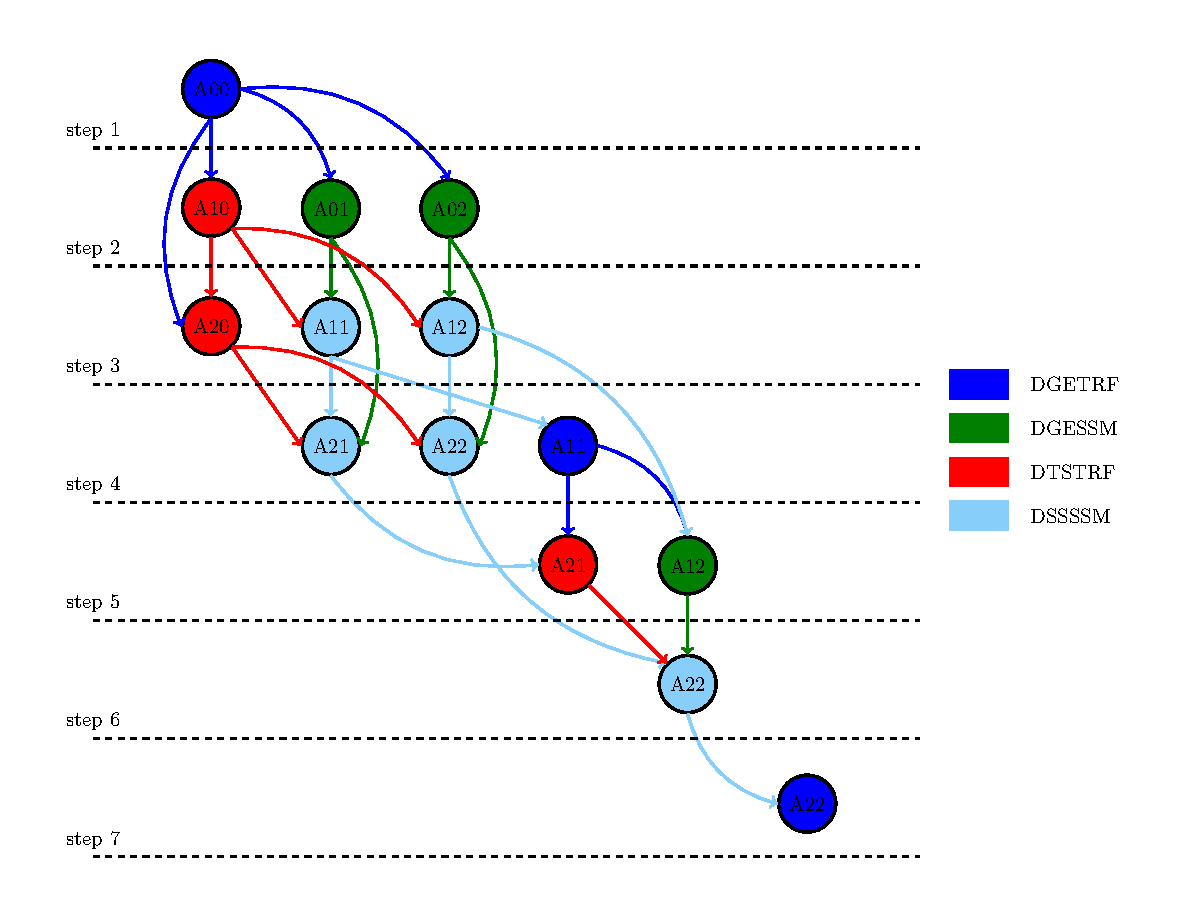
\includegraphics[width=0.8\columnwidth]{figures/lu_task_graph_3x3}
\caption{\emph{Job} graph for tiled LU 3x3 example.}
\label{fig:lu_task_graph_3x3}
\end{figure}

\paragraph{}
	\textbf{Tiled LU}: We have implemented an LU factorization kernel using the Tiled LU algorithm as described in
~\cite{Buttari:2009:CPT:1486274.1486415}.  Figure~\ref(lst:tiledLUseq) shows a simplified version of the tiled
LU algorithm written in C++ style. All arrays are organized in tiles, each tile is a smaller sub array.  Array
\emph{A} is the input array.  In the first step an LU factorization is run on tile \emph{A[k][k]} (\emph{dgetrf} 
function).  The resulting arrays are the lower triangular \emph{L}, the upper triangular \emph{U}, both of which 
are stored in \emph{A[k][k]}, and the transmutation matrix \emph{P[k][k]}.  
The \emph{dgessm} function applies the \emph{L} and 
\emph{U} transformations on all tiles on row k, updating tiles \emph{L[k][k...TOTAL\_TILES]}. \emph{dtstrf}
function performs a block LU factorization on the array formed by coupling the upper triangular part of
\emph{A[k][k]} with \emph{A[k][k]}.
This function returns an upper triangular array, stored in \emph{A[k][k]}, a lower triangular array 
stored in \emph{A[m][k]} and a permutation array P[m][k].  The \emph{dssss} function updates the subarray
formed by tiles \emph{A[k+1...TOTAL\_TILES][k+1...TOTAL\_TILES]} by applying the  transformation computed by \emph{dtstrf}
of the coupled array of the upper triangular part of emph{A[k][n]} and array emph{A[m][n]}.  For the kernels \emph{dgetrf},
\emph{dgessm}, \emph{dtstrf} and \emph{dssssm}, we use the implementation found in the Plasma project
~\cite{1742-6596-180-1-012037}.
	
\paragraph{}
	Figure~\ref{lst:tiledLUpar} shows a simplified version of our parallel implementation.  Figure \ref{fig:3x3lu_example}
shows how the different kernels are applied at each tile for every step.  It also shows how different tiles are depended
upon each other.  The example here is an array that contains 3x3 tiles.  The master process 
starts by executing the \emph{dgetrf}  function.  As soon as it completes, we can apply 
the \emph{dgessm} function on the rest of the tiles on row k (k being the step index we are currenlty working on).
Function \emph{dgessm} only requires the L and U factors from \emph{dgetrf} applied on A[k][k], thus we can issue them 
asynchronously, since all dependencies are met.
We use here a special array of futures \emph{fA} to hold the return value \emph{dgessm}.   
Next, we apply the blocking LU transformation (\emph{dtstrf}) on the rest of the tiles on column k.  Here, because
each \emph{dtstrf} requires the updated A[k][k] tile from the previous application of \emph{dtstrf}, we cannot issue
them in asynchronously.  Instead, after running a \emph{dtstrf} we immediately issue asynchronous calls to \emph{dssssm}.
This function needs to wait from the \emph{dtstrf} that is applied on the first tile on the row, for the \emph{dgessm}
function that will be applied on the first tile of the column, and from the previous, if any, application of \emph{dgessssm}
on the tile just above the current one, that \emph{dgessssm} is applied.  Because \emph{dssssm} modifies two arrays, we use
a struct to represent the coupling of tile A and the upper triangular array U.  The variable cpldAU, is an array of futures
of that struct type.  The parallelization strategy described, allows us to work on each column asynchronously.  
Figure \ref{fig:lu_task_graph_3x3} shows the \emph{job} graph for the Tiled LU 3x3 example.  \emph{Job}s on the same 
step can run in parallel.  The arrows represent the data dependencies among the \emph{jobs}.  Note, that in figure
\ref{fig:3x3lu_example} steps 4 and 5 can be merged, since all data dependencies on tile A11 should have been resolved.
We run the tiled LU kernel for and array of 2000x2000 elements and block size of 200x200 elements.


\begin{figure}[!ht]
\begin{lstlisting}
/* a sequential qs */
void QsSequential(vector<double>& array, const long left, const long right){
    if(left < right){
        const long part = QsPartition(array, left, right);
        QsSequential(array,part + 1,right);
        QsSequential(array,left,part - 1);
    }
}
 
/** A task dispatcher */
class quicksort {
public:
	quicksort() {};
	~quicksort() {};
	vector<double> operator()(vector<double> array, const int deep) {
		const int left = 0;
		const int right = array.size()-1;
    if(left < right){
        if(array.size() > min_unit) {
            const long part = QsPartition(array, left, right);
 						vector<double> subarrA((right)-(part+1)+1), subarrB(part-1-left+1);
						Copy(subarrA, array, part+1, right+1);
						Copy(subarrB, array, left, part);
						quicksort qsort;
						future<vector<double> > res1, res2;
						res1 = async2(subarrA.size(), qsort, subarrA, deep-1);
						res2 = async2(subarrB.size(), qsort, subarrB, deep-1);
            subarrA = res1.get();
            subarrB = res2.get();
						Merge(array, subarrB, subarrA);
        }
        else {
            const long part = QsPartition(array, left, right);
            QsSequential(array,part + 1,right);
            QsSequential(array,left,part - 1);
        }
    }
		return array;
	}
};

\end{lstlisting}
\caption{A quicksort implementation using the distributed futures interface}
\label{lst:quicksort}
\end{figure}


\begin{figure}[!ht]
\begin{lstlisting}
for(int k = 0; k < TOTAL_TILES; k++) {
	dgetrf(A[k][k], P[k][k]);
	for(int n = k+1; n < TOTAL_TILES; n++) {
		dgessm(A[k][n], A[k][k], P[k][k])
	}
  for(int m = k+1; m < TOTAL_TILES; m++) {
		dtstrf(A[k][k], A[m][k] , P[m][k]);
  	for(int n=k+1; n < TOTAL_TILES; n++) {
			dssssm(U[k][n], A[m][n], L[m][k], A[m][k], P[m][k]);
		}
	}
}

\end{lstlisting}
\caption{The tiled LU kernel implementation}
\label{lst:tiledLUseq}
\end{figure}


\begin{figure}[!ht]
\begin{lstlisting}
for(int k = 0; k < TOTAL_TILES; k++) {
	A[k][k] = cpldAU[k][k].get().A;
	dgetrf(A[k][k], P[k][k]);
	for(int n = k+1; n < TOTAL_TILES; n++) {
		A[k][n] = cpldAU[k][n].get().A;
		fA[k][n] = async(dgessm, A[k][n], A[k][k], P[k][k]);
	}
  for(int m = k+1; m < TOTAL_TILES; m++) {
		A[m][k] = cpldAU.get().A;
		dtstrf(A[k][k], A[m][k].get() , P[m][k]);
  	for(int n=k+1; n < TOTAL_TILES; n++) {
			if(m == k+1)
				A[k][n] = fA[k][n].get();
			else
				A[k][n] = cpldAU.get().U;
			A[m][n] = cpldAU.get().A;
			cpldAU[m][n] = async(dssssm, A[k][n], A[m][n], L[m][k], A[m][k], P[m][k]);
		}
	}
}

\end{lstlisting}
\caption{The tiled LU parallel kernel implementation}
\label{lst:tiledLUpar}
\end{figure}

\begin{figure}[!ht]
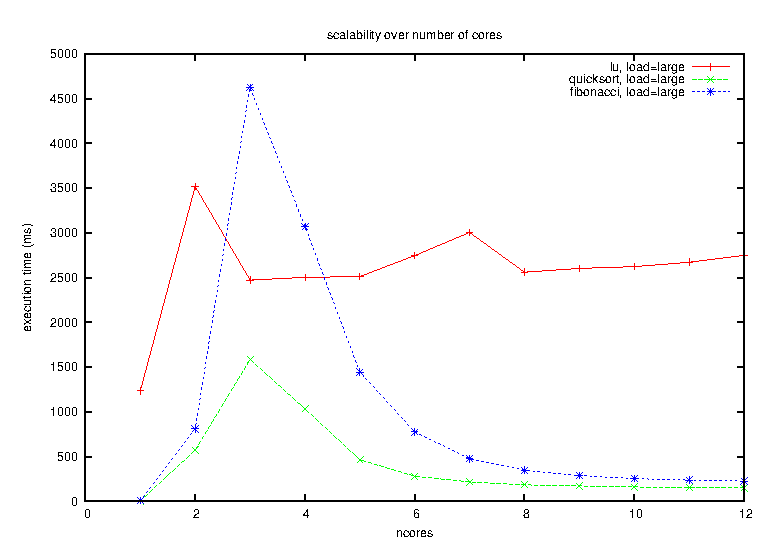
\includegraphics[width=0.7\columnwidth]{figures/apps_scalability}
\caption{Scalability graph for fibonacci, quicksort and LU}
\label{fig:apps_scalability}
\end{figure}

\begin{figure}[!ht]
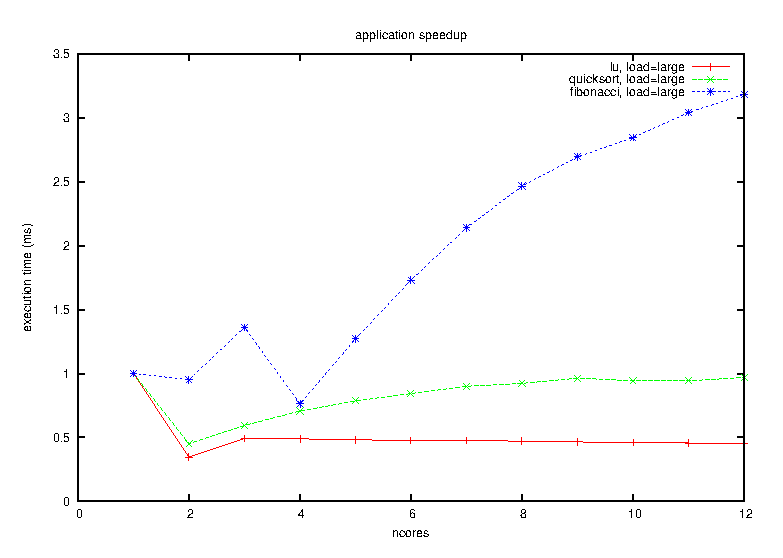
\includegraphics[width=0.7\columnwidth]{figures/apps_speedup}
\caption{Speedup graph for fibonacci, quicksort and LU}
\label{fig:apps_speedup}
\end{figure}

\begin{figure}[!ht]
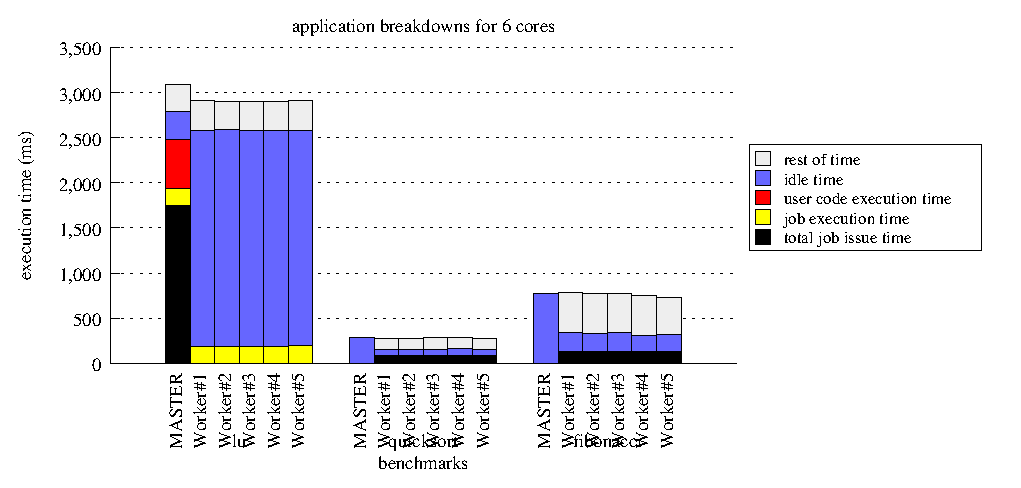
\includegraphics[width=\columnwidth]{figures/app_breakdowns_6cores}
\caption{Breakdowns of master and worker execution time graph for fibonacci, quicksort and LU}
\label{fig:app_breakdowns_6cores}
\end{figure}

\begin{figure}[!ht]
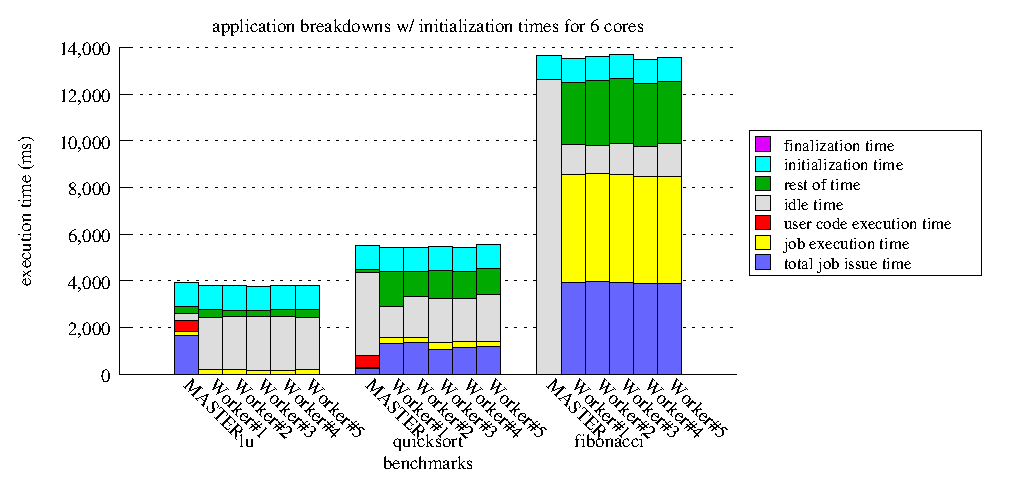
\includegraphics[width=\columnwidth]{figures/app_breakdowns_w_init}
\caption{Breakdowns of master and worker execution time graph for fibonacci, quicksort and LU, with initialization
and finalization times}
\label{fig:app_breakdowns_w_init}
\end{figure}

\paragraph{}
	In figure~\ref{fig:apps_scalability} we report the execution times for running the three applications on the
machine setup we described in section~\ref{sect:eval_intro}.  We measure only the algorithm and no initialization
and finalization times of the runtime system, etc.
We observe that we do not manage to get any speedup 
on quicksort and Tiled LU, on the contrary we get a slowdown (figure~\ref{fig:apps_speedup}).
We get a small speedup in Fibonacci when using more than 4 processes.  
%We also notice a strange
%behaviour of the runtime when running our applications on very few cores. In these cases we have
%noticed an increase in communication when the worker try to return the future value, but we have 
%yet to identify the cause of that issue. \dc{FIXME:say why?}
In figure~\ref{fig:app_breakdowns_6cores} 
we show the breakdowns for the master application and the slaves, for running the applications on 6 cores.
\emph{Job issue time} is the time needed to send a \emph{job} from one process to another. This time includes
time spend in the scheduler, to find the next worker.  It also includes time spend on serializing and sending 
the \emph{job} object and its arguments to a worker process.  \emph{Job execution time} is the time spent on 
running the actual code of the 
\emph{job} that was issued via an \emph{async} call.  \emph{User code time} is the time the master process spends
running code that is not related with the runtime (only for master).  
\emph{Idle time} is time spend waiting to retrieve a future 
value and for the workers, it's also time spent waiting for a \emph{job} to become available in their stacks.
\emph{Rest of time} is the rest of the overhead that is imposed by the runtime.  This fraction of time can be for 
example the time needed to send the return value of the asynchronous execution of a \emph{job} and copies
of objects done after deserialization on the workers.
Figure ~\ref{fig:app_breakdowns_w_init} shows the same breakdowns with figure~\ref{fig:app_breakdowns_6cores}, with 
the addition of initialization and finalization times.  The initialization and finalization include the 
creation and finalization of the communication module (in our experiments that's MPI), creation and destruction
of the shared memory (MPI Windows) and scheduler.  The initialization time is constant on all applications, since
it mainly depends on the number of processes, while the finalization time is negligible.
Compared to the usefull \emph{job execution} and \emph{user code} times, the overhead is much greater.
\emph{Job issue time} or \emph{rest of time} are the greatest sources of 
overhead, while a fair amount of time is also spent on \emph{idle time}.  The \emph{idle time} is more
a concern of the algorithm implentation of each benchmark, and explicitely related to our runtime's overhead.
However, runtime overheads can implicitely be the cause for the \emph{idle time}.  Factors like how \emph{job}s
are distributed among processes and delay in issue time can play a significant role in this.
In order to find the main source of overhead in our system, we used the callgrind tool
to profile our code.  

\paragraph{}
In the Fibonacci application the master spends most of his time waiting for the result on the 
get method.  He does not make any usefull work and only waits for the workers to finish.  Callgrind reports that the
workers spend 52\% running usefull code.  They also spend a high amount (33.3\%) of time on the scheduler trying to 
find the next available worker.  However, out of the 33.3\% only a very small fractio of time (around 3\%) is spend
on actual scheduler work.  The rest 30\% is spend waiting to acquire the lock of the distributed mutex implementation.
One can see that the mutex implementation has a considerable cost.   

\paragraph{}
The master process in quicksort spends 57\% waiting for its workers to complete.  It is again expected, since
most of the work is supposed to be done by the workers, as in Fibonacci.   The workers on the other hand, spend
around 25\% trying to acquire or release locks (distributed mutex) and 32\% on vector allocations.  Half of the
32\% is called from within the serialization routine, which amounts to the total of 16\% of total execution time.
The rest of the vector allocation time is caused by copies of the \texttt{get} method's return value and local
copies of the \emph{async} function's argument, after deserialization.

\paragraph{}
For tiled LU, callgrind reports that the master spends 71\% of its time trying to schedule/send \emph{jobs} to the
workers.  It should be reminded, that all issuing happens by the master in this application, compared to the rest
of our bechmarks.  To quantify this statemen 330 \emph{jobs} are issued by the master.  Except a very small fraction
(around 1\%) is spend exclusively on the serialization routines.  The master also spends 13\% of its time on the 
\texttt{get} method, but 11\% of this is again deserialization of the return values (data send by the workers).  The
serialization routines here are indeed a vast amount of overhead.  This implicitely causes the worker processes to
be idle for a significan amount of time (46\%).  Around 11\% is spend on serialization routines and 15.76 on useful
work.

\paragraph{}
Boost serialization and the distributed mutex library can be identified as the two main causes of overhead in our system.    
Note that Fibonacci makes minimal use of the serialization routines, since it can directly send data (return values and 
argumetns) as MPI datatypes.  Serialization is required only for the \emph{job} object.  Thus fibonacci only suffers from
the overhead caused by the distributed mutex library.  The high cost of the distributed mutex library was expected, and we
tried to use such locks only when completely necessary.  It would be preferable to have a native MPI implementation of 
mutexes, but none of the MPI synchronization primitives can be used to define a critical region.  Moreover, figure 
\ref{fig:app_breakdowns_6cores} shows that even if fibonacci, that there is some performance benefit, the overhead is
considerable.  One can also see that the fibonacci had a lot more useful work to complete compared to tiled LU and 
quicksort.  We believe that the runtime can be only usefull for coarser grain work, with the current implementation.

%\paragraph{\todo{graphs about job issuing over number of workers/jobs issued}}
%\dc{FIXME:say smth about how little the cost for scheduler decision is}

